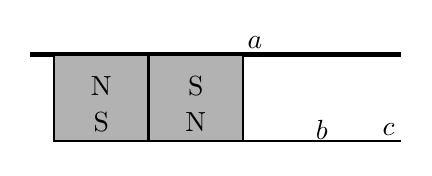
\begin{tikzpicture}[scale=1]
  % rail (thick horizontal bar)
  \draw[line width=2pt] (-0.3,2.0) -- (4.4,2.0);
  % left magnet: N (dark) over S (light)
  \draw[thick,fill=gray!60] (0,0.9) rectangle (1.2,2.0);
  \node at (0.6,1.6) {N};
  \node at (0.6,1.15) {S};
  % right magnet: S (light) over N (dark)
  \draw[thick,fill=gray!60] (1.2,0.9) rectangle (2.4,2.0);
  \node at (1.8,1.6) {S};
  \node at (1.8,1.15) {N};
  \node at (2.55,2.15) {$a$};
  % thin rail continuing to the right
  \draw[thick] (2.4,0.9) -- (4.4,0.9);
  \node at (3.4,1.05) {$b$};
  \node at (4.25,1.05) {$c$};
\end{tikzpicture}
